\documentclass[a4paper,12pt]{memoir}

\usepackage[a4paper,top=2cm,bottom=2cm,left=3cm,right=3cm]{geometry}
\usepackage[utf8]{inputenc}
\usepackage[T1]{fontenc}
% \usepackage[round]{natbib}
\usepackage[english]{babel}
\usepackage{csquotes}
\usepackage[natbib=true]{biblatex}
\usepackage{amsmath}
\usepackage{amssymb}
\usepackage{amsfonts}
\usepackage{amstext}
\usepackage{fancyhdr}
\usepackage[pdftex]{graphicx}
\usepackage{wrapfig}
\usepackage{multicol}
\usepackage{tabularx}
\usepackage{multirow}
\usepackage{caption}
\usepackage{subcaption}
\usepackage[T1,hyphens]{url}
\usepackage[pdfborder={0 0 0 [0 0]}]{hyperref}
\usepackage{color}
\usepackage{siunitx}
\usepackage{booktabs}
\usepackage{setspace}
\usepackage[nottoc,notbib]{tocbibind}
\usepackage[version=4]{mhchem}
\usepackage[numbered]{bookmark}
\usepackage{chngpage}
\usepackage{array}
\usepackage{pdflscape}
\usepackage{titlesec}
\usepackage[a4paper]{couverture/meta-donnees}

\graphicspath{{figures/}}
\addbibressource{/home/webersa/Documents/Articles/bibtex.bib}

\bookmark[page=1,level=0]{Sample document}

\sisetup{per-mode = reciprocal} % reciprocal / symbol 
\DeclareSIUnit\opv{\nmol\per\min\per\cubic\meter}
\DeclareSIUnit\opm{\nmol\per\min\per\ug}

\renewcommand{\hat}{\widehat}


\newcolumntype{P}[1]{>{\centering\arraybackslash}m{#1}}

\newcommand{\E}[1]{\cdot 10^{#1}}
\newcommand{\Var}{\mathrm{Var}} 
\newcommand{\q}[1]{\boxed{\textbf{#1}}}
\newcommand{\ch}{\mathrm{ch}}
\newcommand{\sh}{\mathrm{sh}}
\newcommand{\ta}{\mathrm{th}}
\definecolor{darkred}{rgb}{0.5,0,0}
\definecolor{darkgreen}{rgb}{0,0.5,0}
\definecolor{darkblue}{rgb}{0,0,0.5}
\newcommand{\TODO}[1]{{\color{red}\textbf{TODO: }#1}}
\newcommand{\NOt}{\ce{NO3^-}}
\newcommand{\SOq}{\ce{SO4^2-}}
\newcommand{\NHt}{\ce{NH3}}
\newcommand{\NHq}{\ce{NH4^+}}
\newcommand{\NA}{\ce{NO3NH4}}
\newcommand{\SA}{\ce{SO4(NH4)2}}
\newcommand{\OP}{\text{OP}}
\newcommand{\PM}{\text{PM}}
\newcommand{\PMdix}{\ce{PM10}}
\newcommand{\PMdc}{\ce{PM_{2.5}}}
\newcommand{\PMun}{\ce{PM1}}
\newcommand{\DTTv}{\texorpdfstring{\text{DTT\textsubscript{v}}}{DTTv}}
\newcommand{\AAv}{\texorpdfstring{\text{AA\textsubscript{v}}}{AAv}}
\newcommand{\DTTm}{\texorpdfstring{\text{DTT\textsubscript{m}}}{DTTm}}
\newcommand{\AAm}{\texorpdfstring{\text{AA\textsubscript{m}}}{AAm}}
\newcommand{\OPm}{\texorpdfstring{\text{OP\textsubscript{m}}}{OPm}}
\newcommand{\OPv}{\texorpdfstring{\text{OP\textsubscript{v}}}{OPv}}
\newcommand{\Xg}{{\mathbf{X}^{-g}}}
\newcommand{\OMEGA}{\mathbf{\Omega}}


\hypersetup{
    %    backref=true,               % Permet d'ajouter des liens dans
    %    pagebackref=true,           % les bibliographies
    %    hyperindex=true,            % Ajoute des liens dans les index.
    colorlinks=true,            % Colorise les liens.
    breaklinks=true,            % Permet le retour à la ligne dans les liens trop longs.
    urlcolor=blue,              % Couleur des hyperliens.
    linkcolor=darkred,          % Couleur des liens internes.
    citecolor=darkgreen         % Couleur des citations
}


\author{Samuël Weber}
\title{Source apportionment of the oxidizing potential to the PM sources}

\begin{document}

% \partstyle{madsen}

% \Sethpageshift{26mm}  %%optionnel : à décommenter si besoin pour ajout d'espace afin de center la couvérture horizontalement (valeur par défaut est -5.5mm)
\Sethpageshift{0mm}     %%optionnel : à décommenter si besoin pour ajout d'espace afin de center la couvérture horizontalement (valeur par défaut est -5.5mm)
\Setvpageshift{-17mm}   %%optionnel : à décommenter si besoin pour ajout d'espace afin de center la couvérture verticalement (valeur par défaut est -15.5mm)
%\Universite{}    %%optionnel : à décommenter et à renseigenr si vous voulez changer le non d'université
%\Grade{}         %%optionnel : à décommenter et à renseigenr si vous voulez changer le grade

\Specialite{Océan, Atmosphère, Hydrologie}
\Arrete{25 mai 2016}
\Auteur{Samuël Weber}
\Directeur{Jean-Luc \bsc{Jaffrezo}}
\CoDirecteur{Gaëlle \bsc{Uzu}}    %%optionnel : à décommenter et à renseigenr si présence d'un Co-directeur de thèse
\Laboratoire{Institut des Géosciences de l'Environnement (IGE)}
\EcoleDoctorale{Terre Univers Environnement}
\Titre{Sur les sources du potentiel oxydant des aérosols}
\TitreEN{On the source of the oxydizing potential of aerosols}
% \Soustitre{}      %%optionnel : à décommenter et à renseigenr si présence d'un sous-titre de thèse
\Depot{20 Octobre 2020}
% Commande pour création de nouvelles catégories dans le jury:
%\UGTNewJuryCategory{...NomDeLaCategorie...}{...Definition...}
% Exemple \UGTNewJuryCategory{UGTFamille}{Membre de la famille} que nous ajoutons dans la commande \Jury ci-dessous sous la forme \UGTFamille{Jean Rousseau}{(...titre_et_affiliation...s'il_y_en_a...)}
\Jury{
    \UGTPresident{Didier \bsc{Voisin}}{Professeur, Université Grenoble Alpes -- IGE, Grenoble}
    \UGTRapporteur{Imad \bsc{El Haddad}}{Senior researcher, PSI, Suisse}     %% 1er rapporteur
    \UGTRapporteur{Éric \bsc{Villenave}}{Professeur, Université de Bordeaux -- EPOC, Bordeaux}      %% second rapporteur
    \UGTExaminateur{Matthias \bsc{Beekmann}}{Directeur de recherche, CNRS -- LISA, Paris}   %% 3ème examinateur
    \UGTExaminatrice{Éva \bsc{Léoz-Gardzienda}}{Ingénieure, INERIS, Verneuil-en-hallate}
    \UGTExaminatrice{Nathalie \bsc{Poisson}}{Ingénieure, ADEME, Paris}
    \UGTCoDirectrice{Gaëlle \bsc{Uzu}}{Directrice de recherche, IRD -- IGE}     %% Directeur de thèse
    \UGTCoDirecteur{Jean-Luc \bsc{Jaffrezo}}{Directeur de recherche, CNRS -- IGE}   %% Co-Directeur de thèse s'il y en a
    % \UGTInvite{Cali \bsc{Méro}}{Ingénieur Expert, Laboratoire Pierre Gattaz, Paris} 
}
\MakeUGthesePDG    %% très important pour générer la couverture de thèse


\maketitle

\newpage
% \part*{Acknowledgements}
% \addcontentsline{toc}{part}{Acknowledgements}
% \onehalfspacing
% First of all, I wish to thanks Jean-Luc for supporting me during almost
% two years now. Thanks to introduce me to the very interesting topic of Air
% Quality science.  Also, thanks you very much for the confidence you accorded to
% me and for the great opportunities you offer to me in the past two years and
% chaptericularly for the PhD you proposed to me and I accepted cheerfully. 
%
% Thanks also to you, Gaëlle, for successfully supervising my internship from your
% 3600 meter height in La Paz, Bolivia.  Undoubtedly, between Benjamin in Antarctica
% last year and you in Bolivia this year, it seems that one of my supervisor
% always \emph{have to be} in a cold environment, far away from Grenoble :). 
% Thanks for the ideas, your encouragement and your willingness despite the ocean
% and Amazonia between use!
%
% I also wish to thank the little OP-team: Aude and Céline. Thanks for the rich
% discussions we had about OP and error\dots Good luck with the PCA!
%
% Also, many thank to Didier for the frequent \emph{not so silly questions} and
% sharing ideas with you.
%
% Many thanks also to Dalia for sharing your office with me during this internship
% and answering my newbie questions on atmospheric chemistry and also for your
% biscuits at 4 P.M!
%
% And of course, many thanks to Vincent, Coralie and Lisa and all the others for
% the analyses of the sample and dealing with the caprice of the EC/OC or the
% others silly instruments of the lab!
%
% Finally, I am greatful to Jean-Luc (Besombes), not only for his PAH analyses,
% but also for accepting to be my reviewer.
% \normalsize
%

% Fakepart TableofContent
\tableofcontents
\listoftables
\listoffigures

\part{Introduction}%
\label{cha:introduction}

The Air Quality has become one of the most environmental issue in the past decades. It is
now well-known that the air quality cause dramatic health damage. The CAFE program (Clean
Air For Europe) estimates that the $\PM_{2.5}$ are responsible for a decrease of a
lifetime of 9 months in average in Europe. Another study from~\citet{amann_baseline_2005}
indicates that around 42 000 premature death in France are due to the PM concentration in
the air.  This pollution has a health impact both during a pollution peak (asthma,
vulnerability to disease, etc) and with a chronicle exposition (cancer, pulmonary
infection, cardiovasculary disease, etc).

Nowadays, the regulation of the air quality aims to reduce the population exposition to
the air pollutant. For instance in France since the LAURE law (Loi sur l'Air et
l'Utilisation Rationelle de l'Énergie) in 1996, frequent measurements of the air quality
is mandatory.  To do so, the regulation focuses its guidelines on the total mass of the PM
present in the air.  In 2000 the ecology french minister setups several \emph{Association
Agrées de Surveillance de la Quality de l'Air} (AASQA) which monitor, among other things,
the $\PM_{10}$ and $\PM_{2.5}$ mass in \si{\um\per\cubic\m} in the air.  The current
french regulation imposes a daily maximum concentration of \SI{50}{\ug\per\cubic\m} for
$\PM_{10}$ and \SI{25}{\ug\per\cubic\m} for $\PM_{2.5}$. However, this threshold, and so
the population exposition, is regularly exceeded in some urban cities like Paris, Lyon or
Grenoble, or even in some other place like the Arve Valley in the Alps.
Moreover, the PM term regroup only chaptericle which share a size lower than few micrometers,
but they are highly different in term of chemical composition, shape or physical
properties. It results that some PM may be more biologically active than others.  The
metric of the mass of the PM is then not appropriate as \SI{10}{\um\per\cubic\m} of sugar
will not have the same effect as \SI{10}{\um\per\cubic\m} of mercury for instance.  The
fundamental question for human health is then: do all aerosols have the same health
impact? How can we measure it? 

In the past few years emerged the idea of a new metric: the Oxidant Potential (OP) of the
{PM}. The OP is indeed linked to all the physico-chemical characteristic of the PM: the
shape, the size and the chemical composition.  Moreover, the OP could be linked to a
health impact more easily than the mass.  Indeed, in the human lung anti-oxidant are
present to counteract the oxidative potential of the air (radicals, gases and also
aerosols).  In fact, the OP is a measure of the Reactive Oxygen Species (ROS) carried or
induced by aerosols. When there is an unbalance between the lung anti-oxidant defense and
the ROS, an inflammatory response is observed
\citep{donaldson_oxidative_2003,delfino_potential_2005,li_adjuvant_2009}.  The OP of the
PM is then considered as a promising proxy for Air Quality purpose.  Recently,
\citet{fang_oxidative_2016} coupled measurements of OP and large population
epidemiological analyses and shows a strong correlation between entry in emergency
dechapterment and the OP of the {PM}.
However, such studies are quite recent and present the necessity of further investigations
and rise new questions: how do we measure the {OP}? Could we do it standardly?  Is it
possible to easily measure it?  Will it be useful to understand the dynamic of the sources
and their respective environmental impact?


My internship will be focused on the comprehension of the link between the OP and the
chemistry of the PM and especially to an estimation of the OP contribution by sources of
{PM} in the frame of the ExPOSURE program funded by the ANSES\footnote{ANSES: Agence
    Nationale de Sécurité Sanitaire de l'alimentation, de l'environnement et du travail}.
    Such study is one of the first in the literature and undoubtedly the one associated
    with the biggest sample in the world.  I will first explain some generalities of the
    atmospheric sciences and aerosols (chapter~\ref{chapter:context}). Secondly, I will explain
    the methodology of the study and the sample acquisition (chapter~\ref{chapter:measure}).
    The third chapter is focused on the results obtain during this internship and is split in
    two main sections: the mathematical development of an inversion framework for the
    attribution of the OP to the source (section~\ref{sec:inversionMethod}
    chapter~\ref{chapter:results}) and the results obtained with this new method (the rest of
    the chapter~\ref{chapter:results}).

% To do so, I will follow the workflow given in
% fig.~\ref{fig:workflow_intership}.  The internship is focused on the setup of
% the inversion procedure to attribute an intrinsic OP of the input variable
% (chemical species or emission sources), this is the \emph{inversion} box in the
% figure.  The goal is to attribute an intrinsic OP per \si{\ug} of species or per
% \si{\ug} of emission from a source.  
%
% The speciation of the aerosol chemistry and the OP measurement are discussed in
% the section~\ref{sec:analysis} in chapter~\ref{chapter:measure}.  The PMF model is
% briefly explain in the section~\ref{sec:PMF} in chapter~\ref{chapter:measure} and was
% run by several persons (Dalia Salameh for the site of the SOURCES program,
%     Alexandre Sylvestre for the sites of Nice, Florie Chevrier for the sites of
% the DECOMBIO program). The methodology of the inversion is detailed in the
% section~\ref{sec:inversionMethod} in chapter~\ref{chapter:results}.
%


\part{State of the art}%
\label{cha:state_of_the_art}

\section{The atmosphere}%
\label{sec:the_atmosphere}

\subsubsection{The atmosperic boundary layer}%
\label{ssub:the_atmosperic_boundary_layer}
The first boundary layer of the atmosphere (ABL) is the layer of the atmosphere
which is directly and strongly impacted by the surface of the Earth. The ABL is
about \SI{15}{\kilo\m} height and contains more than 80 \% of the total air mass of
the atmosphere.  The ABL is then the most important layer when dealing with
pollution as all the emission (natural and anthropogenic) from the surface
accumulate into it, conditioning the air we breathe both in the gaseous phase
(\ce{CO} for instance) or the solid phase in suspension in the air (called
aerosols or chaptericulate matter (\PM)).  It is then now well-known that the human
activities bring a large variety of pollutant in the atmosphere, both at local
or large scale.  These pollutants are a key issue when for the climatology and
for the environmental science as they impacted the energy budget of the Earth
and the chemistry of the atmosphere.  This internship is focused on the
chaptericulate matter and their sources in the atmosphere. 

\section{Atmospheric chaptericulate matter}%
\label{sec:atmospheric_chaptericulate_matter}
\subsubsection{A brief description of an aerosol}%
\label{ssub:a_brief_description_of_an_aerosol}

An aerosol is a solid or liquid chaptericle in suspension in the air.  Some
typology of aerosols exist and are differentiated thanks to their size and
chemical composition.  Their size varies from nanometer to micrometers, with 3
main \emph{mode} depending mainly on their origin.  However, the relative
importance of each of theses 3 modes vary if we consider the mass (proportional
to the volume), the surface or the number of aerosols (see
fig.~\ref{fig:aerosolDistribution}). 

\begin{figure}[h]
    \centering
    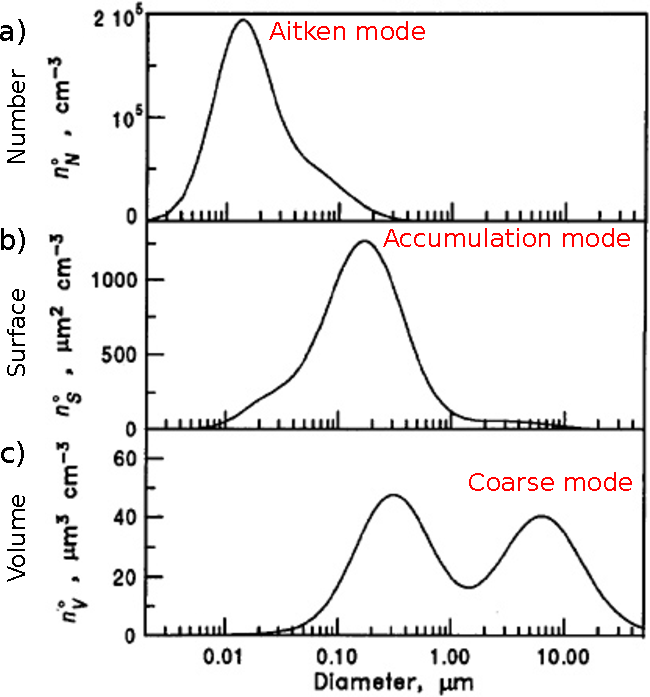
\includegraphics[width=0.4\textwidth]{aerosolDistribution.pdf}
    \caption{\textbf{(a)} Aerosol number, \textbf{(b)} surface area, and
        \textbf{(c)} volume for a typical trimodal aerosol
        distribution.  Figure adapted from the
    book of~\citet{seinfield_atmospheric_1998}.}
    \label{fig:aerosolDistribution}
\end{figure}

An aerosol is composed of several chemical species like ions (\SOq, \NOt, \ce{Na+},
\ce{Cl-}, \ce{Mg^2+}, etc), metals (\ce{Cu}, \ce{Al}], \ce{Ti}, \ce{Ca}, etc), and organics species
(cellulose or other sugar, “black carbon”, hopanes, etc).  They come from different
sources: natural like volcano, biology, desert (resuspension due to the wind) or marine
spray for instance and anthropogenic like traffic exhaust, brake wear, industry, biomass
burning or agriculture.  Each of these sources emits different species, in different
quantity and in different place of the atmosphere and of the Earth and with different
shape as shown in fig.~\ref{fig:micrography}.  However, the average lifetime of an aerosol
is from hour to week, and then can impact a wide area.  For instance the black carbon
emitted in developed countries is a major issue for the ice melt in the Artic's iceshelf.
More generally, aerosols are a key parameter in the climate system as they interact with
the Solar and Earth radiation, act as cloud/ice condensation nucleii and chaptericipate to
the precipitation process \citep{boucher_clouds_2013}.

The nomenclature of the PM is linked to their size: \PMdix~covers all chaptericles with a
diameter lower than \SI{10}{\um}, \PMdc~with a diameter lower than \SI{2.5}{\um} and
\PMun~with a diameter lower than \SI{1}{\um}.  These categories do not have the same
chemical composition nor shape as they reflect different source or different process in
place in the atmosphere. Indeed, aerosols can react with the gas (\ce{SO2},
\ce{NO2}, \ce{NH3} for instance), radiation or radicals (the so call hydroxyl radical
\ce{HO^.}) or even with other aerosols and form new species or bigger aerosols. We then
call this aerosol \emph{secondary aerosol} as it do not reflect a primary source but
reaction in the atmosphere.

\begin{figure}[h]
    \centering
    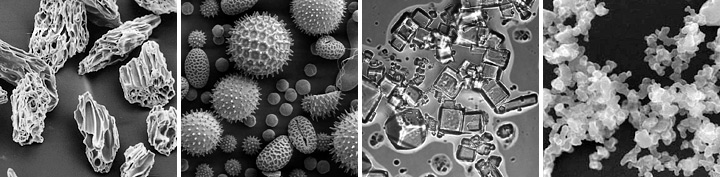
\includegraphics[width=0.8\textwidth]{aerosol_micrographs.jpg}
    \caption{Scanning electron microscope
        images (not at the same scale) showing the wide variety of aerosol shapes. From
        left to right: volcanic ash, pollen, sea salt, and soot. Micrographs from USGS,
        UMBC (Chere Petty), and Arizona State University (Peter Buseck).  Credit: NASA
        earthobservatory
    \url{https://earthobservatory.nasa.gov/Features/Aerosols/}.}
    \label{fig:micrography}
\end{figure}

\section{The oxidative potential}%
\label{sec:the_oxidative_potential}

\part{Database at the IGE}%
\label{cha:database_at_the_ige}


\part{Source apportionment of PM}%
\label{cha:source_apportionment_of_pm}

\chapter{Chemical signature of the sources}%
\label{prt:chemical_signature_of_the_sources}

\chapter{Source apportionment model}%
\label{prt:source_apportionment_model}

\section{Direct modeling}%
\label{sec:direct_modeling}

\subsection{Lagrangian or dispersion model}%
\label{sub:lagrangian_or_dispersion_model}

\subsection{Deterministic chemistry transport model (CTM)}%
\label{sub:deterministic_chemistry_transport_model_ctm_}

\section{Receptor model}%
\label{sec:receptor_model}

\subsection{Chemical mass balance (CMB)}%
\label{sub:chemical_mass_balance_cmb_}

\subsection{Principal component analysis (PCA)}%
\label{sub:principal_component_analysis_pca_}

\subsection{Positive matrix factorization (PMF)}%
\label{sub:positive_matrix_factorization_pmf_}





\part{Methodology for the attribution OP to a PM source}%
\label{cha:methodology_for_the_attribution_of_intrisinc_op_to_a_pm_source}

\part{Application to 15 sites in France}%
\label{cha:application_to_15_sites_in_France}

\part{Spatio-temporal modelizing}%
\label{cha:spatio_temporal_modelizing}

% Fakepart Bibliography
\pagebreak
\addcontentsline{toc}{chapter}{Bibliography}
\printbibliography
\pagebreak

\part*{Appendix}%
\label{cha:appendix}


\addcontentsline{toc}{chapter}{Appendix}
\appendix
\setcounter{table}{0}
\setcounter{figure}{0}
\setcounter{equation}{0}
\renewcommand{\thetable}{\thesection-\arabic{table}}
\renewcommand{\thefigure}{\thesection-\arabic{figure}}
\renewcommand{\theequation}{\thesection-\arabic{equation}}

\end{document}
